%%
%% This is file `sample-acmsmall-conf.tex',
%% generated with the docstrip utility.
%%
%% The original source files were:
%%
%% samples.dtx  (with options: `acmsmall-conf')
%% 
%% IMPORTANT NOTICE:
%% 
%% For the copyright see the source file.
%% 
%% Any modified versions of this file must be renamed
%% with new filenames distinct from sample-acmsmall-conf.tex.
%% 
%% For distribution of the original source see the terms
%% for copying and modification in the file samples.dtx.
%% 
%% This generated file may be distributed as long as the
%% original source files, as listed above, are part of the
%% same distribution. (The sources need not necessarily be
%% in the same archive or directory.)
%%
%% The first command in your LaTeX source must be the \documentclass command.
\documentclass[acmsmall,nonacm]{acmart}
\settopmatter{printacmref=false} % Removes citation information below abstract
\renewcommand\footnotetextcopyrightpermission[1]{} % removes footnote with conference information in first column
%\pagestyle{plain}

%%
%% \BibTeX command to typeset BibTeX logo in the docs
\AtBeginDocument{%
  \providecommand\BibTeX{{%
    \normalfont B\kern-0.5em{\scshape i\kern-0.25em b}\kern-0.8em\TeX}}}
    
\definecolor{beaver}{RGB}{215, 63, 9}
\definecolor{luminance}{RGB}{255, 181, 0}


\usepackage{amsmath}
\usepackage[mathletters]{ucs}
\usepackage[utf8x]{inputenc}
\usepackage{multicol}
\usepackage{comment}
\usepackage{graphicx}
\usepackage{parskip}
%%\setlength{\parskip}{0.2em}

%% Rights management information.  This information is sent to you
%% when you complete the rights form.  These commands have SAMPLE
%% values in them; it is your responsibility as an author to replace
%% the commands and values with those provided to you when you
%% complete the rights form.
%\setcopyright{none}
%\copyrightyear{}
%\acmYear{}
%\acmDOI{}

%% These commands are for a PROCEEDINGS abstract or paper.
%\acmConference[Woodstock '18]{Woodstock '18: ACM Symposium on Neural
%  Gaze Detection}{June 03--05, 2018}{Woodstock, NY}
%\acmBooktitle{Woodstock '18: ACM Symposium on Neural Gaze Detection,
%  June 03--05, 2018, Woodstock, NY}
%\acmPrice{15.00}
%\acmISBN{978-1-4503-XXXX-X/18/06}


%%
%% Submission ID.
%% Use this when submitting an article to a sponsored event. You'll
%% receive a unique submission ID from the organizers
%% of the event, and this ID should be used as the parameter to this command.
%%\acmSubmissionID{123-A56-BU3}

%%
%% The majority of ACM publications use numbered citations and
%% references.  The command \citestyle{authoryear} switches to the
%% "author year" style.
%%
%% If you are preparing content for an event
%% sponsored by ACM SIGGRAPH, you must use the "author year" style of
%% citations and references.
%% Uncommenting
%% the next command will enable that style.
%%\citestyle{acmauthoryear}

%%
%% end of the preamble, start of the body of the document source.
\begin{document}

%%
%% The "title" command has an optional parameter,
%% allowing the author to define a "short title" to be used in page headers.
\title{Password Strength Meters}

%%
%% The "author" command and its associated commands are used to define
%% the authors and their affiliations.
%% Of note is the shared affiliation of the first two authors, and the
%% "authornote" and "authornotemark" commands
%% used to denote shared contribution to the research.
\author{David Chen}
\email{chend2@oregonstate.edu}
\affiliation{%
  \institution{Oregon State University}
  \city{Corvallis}
  \state{Oregon}
  \country{USA}
  \postcode{97331}
}

\author{Abdullah Saydemir}
\email{saydemia@oregonstate.edu}
\affiliation{%
  \institution{Oregon State University}
  \city{Corvallis}
  \state{Oregon}
  \country{USA}
  \postcode{97331}
}

\author{Lindy Voss}
\email{vossli@oregonstate.edu}
\affiliation{%
  \institution{Oregon State University}
  \city{Corvallis}
  \state{Oregon}
  \country{USA}
  \postcode{97331}
}


%%
%% By default, the full list of authors will be used in the page
%% headers. Often, this list is too long, and will overlap
%% other information printed in the page headers. This command allows
%% the author to define a more concise list
%% of authors' names for this purpose.
\renewcommand{\shortauthors}{Chen, Voss, \& Saydemir}

%%
%% The abstract is a short summary of the work to be presented in the
%% article.
\begin{abstract}
    Passwords are integrated into our everyday lives, whether it be accessing social media accounts, logging onto computers and unlocking our phones, or protecting our financial/banking information. Despite how important they are, people still create and use weak passwords that can easily be cracked by hackers for malicious intent. In this article, we looked into entropy calculations, different cracking techniques to better understand how passwords are cracked, and introduce several better password creation. We also demonstrated ways to make those strong passwords more memorable. With these methods, it will be easier to create a password that is less likely to be cracked without compromising the memorability. We conclude the paper by analyzing the scalability of the methods and suggest a solution to password management issue considering the fact that reusing the same strong password will cause issues.
\end{abstract}

%%
%% The code below is generated by the tool at http://dl.acm.org/ccs.cfm.
%% Please copy and paste the code instead of the example below.
%%
\begin{CCSXML}
<ccs2012>
   <concept>
       <concept_id>10002978.10003029.10011703</concept_id>
       <concept_desc>Security and privacy~Usability in security and privacy</concept_desc>
       <concept_significance>500</concept_significance>
       </concept>
   <concept>
       <concept_id>10002978.10002991.10002992</concept_id>
       <concept_desc>Security and privacy~Authentication</concept_desc>
       <concept_significance>300</concept_significance>
       </concept>
   <concept>
       <concept_id>10002978.10003029</concept_id>
       <concept_desc>Security and privacy~Human and societal aspects of security and privacy</concept_desc>
       <concept_significance>500</concept_significance>
       </concept>
   <concept>
       <concept_id>10002978.10002979.10002983</concept_id>
       <concept_desc>Security and privacy~Cryptanalysis and other attacks</concept_desc>
       <concept_significance>100</concept_significance>
       </concept>
 </ccs2012>
\end{CCSXML}

\ccsdesc[500]{Security and privacy~Usability in security and privacy}
\ccsdesc[300]{Security and privacy~Authentication}
\ccsdesc[500]{Security and privacy~Human and societal aspects of security and privacy}
\ccsdesc[100]{Security and privacy~Cryptanalysis and other attacks}

%%
%% Keywords. The author(s) should pick words that accurately describe
%% the work being presented. Separate the keywords with commas.
\keywords{security, password, memorability}

%% A "teaser" image appears between the author and affiliation
%% information and the body of the document, and typically spans the
%% page.

%%
%% This command processes the author and affiliation and title
%% information and builds the first part of the formatted document.
\maketitle

\section{Introduction}
Passwords are used nowadays as the first line of defense to protect information along with other options \cite{ma_2010}. Though passwords are meant to be solid and secure, they have flaws that can be easily exploited. In 2019, nearly 1 terabyte of user account data including passwords previously collected from Yahoo and some other website breaches were for sale \cite{hunt_2019}. Hashes of mostly used passwords, including those from Yahoo!, get uploaded to haveibeenpwned.com for the public to check whether their passwords were breached. Among 700 million unique passwords, two of the most commonly used were “123456” (more than 24 million times) and “password” (more than 3 million times) which can be broken in virtually zero time.


To prevent these from happening, the websites benefit from password composition rules (e.g. password must contain both lowercase and uppercase letters). Studies show that enforcing these rules helps users to choose stronger passwords \cite{shay_2010}. However, this also increases user fatigue since the average number of website accounts a single user has is around 25 \cite{lee_2014,waugh_2012}  and continues to increase. This exhaustion leads to people creating one (or a few) strong passwords, often reusing those passwords across many websites \cite{das_2014} and preserving them for long periods \cite{bhagavatula_2020,florencio_2007}. Moreover, only one third of people change their password after a breach and most of them change their passwords to weaker or equally strong ones \cite{bhagavatula_2020}. This leads to large collections of passwords (that are gathered on the internet) being used in brute force attacks over and over again, often with some success due to all of the unchanged passwords. There are also highly specific versions of dictionaries used in these attacks that are categorized according to attack type, platform, website, language and even to geological location.


The problem with strong and secure passwords is nobody can remember them. Especially with the amount of websites and accounts people hold nowadays. People are told to create strong passwords and in order to do that they have to avoid short passwords, birthdays, names, places, dictionary words, and the list goes on \cite{lee_2014}. Basically you are not supposed to use anything remotely memorable. Say you come up with a strong password like Jf5ruEf392HQlx and somehow memorize it. Well you can only use that for one account and the rest all have to be different but just as strong \cite{rubenking_2021}. This begs the big question of how do you create a strong password (for each account) that is realistic to memorize for practical use? There are tools and different tricks that have been found to work to help people balance these two very important factors when deciding on a password so they can not only remember their passwords, but also keep their information safe.

Therefore, in this article, we propose the following contributions:

\begin{itemize}
\item We will have a look at password entropy calculation to understand what dictates the strength of passwords.
\item We introduce different password cracking techniques used to understand how passwords are being solved to better adapt new passwords to prevent cracking
\item We introduce password creation techniques and guidelines, and discuss their strengths in relation to password entropy.
\item We introduce memorable passwords that are still strong to resist brute force / dictionary attacks.
\end{itemize}

In the next section, we will present an overview of concepts that are helpful to understand how a strong password is created.

\section{Concepts}

\subsection{Password} \label{password}

Password, common name for the term \emph{Memorized Secret Authenticator}, is a secret key that the user randomly selects and memorizes \cite{nist_2020}. Passwords must have enough complexity and secrecy that an adversary would be unable to guess or discover the secret value. If the password consists only of numbers it can be referred as PIN.

There are two other important definitions. \emph{Neutral Passwords} are those do not contain any information about the user whereas \emph{Biographic Passwords} are those that do contain information about the user \cite{Kavrestad_2019}.

\subsection{Passphrase} \label{passphrase}

Passphrase is a memorized secret that consists of sequences of words or phrases. It is usually longer than password to add more security \cite{passphrase_def}.

\subsection{Password Entropy / Strength} \label{entropy}
Password entropy is a measurement how strong a password is. It is used to estimate effectiveness of a password against guessing or brute-force attacks. Higher entropy means stronger passwords whereas lower entropy means weaker. It depends on the complexity and length \cite{hu_2018}.

To put it in mathematical way, let's say \emph{P} is a password of length \emph{l} and consists of characters in alphabet $\Sigma$ size of which is equal to \emph{N}. That is, \emph{N} = |$\Sigma$| . Then, the entropy \emph{E} of this password \emph{P} is calculated with the following equation :
\begin{equation} \label{eq:1}
E = \log_2 N^l = l \cdot \log_2 N
\end{equation}

\begin{table}[ht!]
 \begin{tabular}[c]{| l  c  c |} 
\hline 
 Character Set & Elements & Set Size \\
 \hline\hline
 Digits & 0-9 & 10  \\ 
 \hline
 Latin letters (lowercase) & a-z & 26 \\
 \hline
 Latin letters (uppercase) & A-Z & 26  \\
 \hline
 Alphanumeric & a-z $\cup$  0-9 & 36  \\
 \hline
 Alphanumeric and Uppercase & a-z $\cup$ A-Z $\cup$ 0-9 & 62 \\  
 \hline
 Symbols (US keyboard) & $~!@\#\$\%\&*()-+=[]\{\}|;$ etc. & 32  \\
 \hline
 \end{tabular}
 \caption{Most Used Password Sets}
 \label{tab:sets}
\end{table}

We can directly deduce that increasing either of \emph{L} or \emph{N} creates passwords that have higher entropy. Therefore, to create a stronger password user should either choose a larger set of characters or make the password longer. It is obvious that for some specific numbers, entropy of longer password from a smaller set can be similar to entropy of the shorter password from a larger set. For example, let $\emph{P}_1$ a password that consists of digits and its length is 11. Let $\emph{P}_2$ another password that consists of lowercase Latin letters and its length is 8. If we calculate the entropy of both using set sizes given in \autoref{tab:sets}:
\begin{align*}\label{eq:p1p2calc}
    \emph{E}_1 = \log_2 10^{11} &= 11 \cdot \log_2 10 = 11 \times 3.32 &\emph{E}_1 \approx 36.5 \\
    \emph{E}_2 = \log_2 26^8  &= 8  \cdot \log_2 26   = 8 \times 4.70 &\emph{E}_2 \approx 37.6
\end{align*}

\noindent we can see that there is not much difference between the entropy of the two passwords. However, it is important to note that entropy itself is \textbf{not} all it matters. Consider the same passwords $\emph{P}_1$ and $\emph{P}_2$ but this time let $\emph{P}_1$ be the string "46583159027" and $\emph{P}_2$ be the string "password". In this case, $\emph{P}_2$ is extremely weak and it can be broken in virtually zero time since it appears in leaked password lists.

Therefore, aside from the two parameters of \autoref{eq:1}, \emph{unpredictability}  is another factor that has an effect on password strength. We will talk about this concept in detail in \autoref{creation}.

Some adjustments can be made on password entropy calculation by making assumptions on the strength of the attackers. In this article, we will use the \autoref{eq:1} without any adjustments since assumptions may or may not hold true for each case. 

\subsection{Password Cracking-Techniques} \label{cracking}

In order to know how to to best create a strong memorable password, it is important to know how many passwords are cracked. There are many different types of techniques that a hacker can use to figure out one's passwords. Each technique share the same end goal, but their execution differs. These techniques fall under three different categories of cracking: password-focused, human-focused, and computer focused. This document will only concern the password-focused techniques. These technique focuses on the password themselves, cracking the characters or the words used in each user's password. 

Different techniques have different success rates and execution difficulty. For example, phishing is a technique where a user is tricked into clicking or downloading a malicious file, where malware is executed. Normally, these disguise themselves as emails telling the user to take action of some sort \cite{walker_2020}. This technique is difficult to execute because it is based off the user's ignorance to work, but the times that it does the hacker would be able to easily get passwords and other information from the user. 

\newpage
For the password-focused category, they generally contain techniques that aren't too difficult to achieve, but have a lower chance of success than techniques in the other categories. It also has more tools that average people can download and use themselves to crack passwords. There are many tools out there. \emph{Hashcat} is one example of these tools. Hashcat is a tool that does one of the techniques that will be mentioned below, and is available to download to the general public. It can be used both licitly and illicitly, such as a system admin checking the security of their client's passwords, or a hacker moving through a system and gaining admin privileges \cite{porup_2020}. The following are some examples of password-focused cracking techniques.

\subsubsection{Brute Force Attack}
Brute Force is the most common and simplest technique used by hackers. It is a technique where an algorithm is used to try as many possible keyword and password combinations to gain access to the system and/or file \cite{kaspersky_2021}. These generally work best on simpler passwords, such as "\emph{password}", "\emph{123456}", "\emph{qwerty}", and possible iterations, "\emph{p@ssword}", "\emph{PaSsWoRd}", etc.

\subsubsection{Dictionary Attack}
Dictionary attacks are a type of brute force attacks, except it heavily relies on \emph{cracking dictionaries}, which are lists that contain the most common passwords, word combinations, and dictionary words \cite{walker_2020}. They may also contain credentials from previous hacks in other systems. 

\subsubsection{Mask Attack}
Mask attacks are similar to the standard brute force attacks, except they rely on scanning through specific characters and letters in a specific pattern. For example, if a hacker knows that the password is an 8 character password that starts with an uppercase letter, followed by three lowercase letters, where the last four characters will be a number or a special character, then he just needs to set up an algorithm that scans all the characters needed in that specific arrangement \cite{jake_2018}.

However, the drawback of brute force and dictionary/masks attacks is that the time to crack the password is based off the length and complexity of the password, which relates directly to entropy. As stated in \ref{entropy}, it helps estimate the effectiveness of the password against brute force attacks. The higher the entropy of a password, the longer it takes for the algorithm to be able to crack it. It's possible for some of the stronger passwords to take years to crack, depending on it's length and complexity.

\section{Password Creation Techniques} \label{creation}

We know what contributes to password strength and how adversaries try to crack passwords. Hence, we can use these knowledge to create strong passwords. However, we need to know the essential requirements, dos and don'ts.

According to the latest NIST guidelines \cite{nist_2020}, a password must consist of at least 8 characters and users should be encouraged to use as lengthy password as possible, within reason. On the other side passwords should not include the following items:

\begin{itemize}
\item Passwords that are inside leaked password lists e.g. "password" 
\item Dictionary words e.g. "!-summer?5"
\item Repetitive or sequential characters e.g. "aaaaaaaa" or "abcd1234"
\item Context-specific words e.g. name of the service, username or derivatives
\end{itemize}

Having these in mind, let's see couple of methods to create strong passwords.

\subsection{Strong Passwords} \label{strong}

\subsubsection{Traditional Method} \label{creation-traditional}

There are several studies that show enforcing or suggesting password composition rules increase the password strength \cite{shay_2010, shay_2015}. Services usually provide compositions rules and often enforce the user to create a password that comply with these rules. The suggestions vary across services but most common ones are as follows:

\begin{itemize}
\item Password length should be at least 12
\item Password should include uppercase/lowercase letters, symbols and numbers
\item Password should not include obvious substitutions $S$ ${\displaystyle \rightarrow }$ $\$$
\end{itemize}

Prompted with these, what most users do is creating a sequence of string (meaningful or meaningless) and further substituting some symbols/numbers if required. Though this method, Traditional Method, is one of the most primitive methods used in password composition, it is still capable of offering strong passwords.

For example, let "\emph{latexcoroutine}" be the base string. A possible symbol and number substitution would be "$L/-\backslash t[-;CO2ine$". Therefore, the entropy of the password would be:
\begin{align*}
    \emph{E} = \log_2 94^{14} &= 14 \cdot \log_2 94 = 14 \times 6.55 &\emph{E} \approx 91.7
\end{align*}

\subsubsection{Passphrase Method} \label{creation-passphrase}

As we talked in \autoref{passphrase}, passphrases are lengthy passwords that consist of multiple words or phrases. \autoref{eq:1} specifies that increasing length of the password directly contributes to password entropy; therefore, increases the password strength. Furthermore, NIST suggests using passwords as lengthy as possible. Passphrase method tries to achieve the highest password strength by greedily increasing the length.

Words that form the passphrase must be random, varied, and the passphrase must be neutral (i.e. non-biographic) \cite{nist_2020,Kavrestad_2019}. To accommodate the random word selection, Diceware \cite{reinhold_2021} offers a method and multiple word lists consisting of more than 7000 words. Random passphrase creation method is as follows:

\renewcommand{\labelenumi}{\arabic{enumi}.}
\begin{enumerate}
    \item Roll a die five times (or five dices at once) and record the numbers 
    \begin{align*}
        \emph{4  2  4  6  4}
    \end{align*}
    \item Concatenate the result and find the corresponding word for your number in the word list 
    \begin{center}
        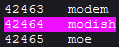
\includegraphics{modish1}
    \end{center}
    
    \item Do this until you have sufficiently long passphrase (5-word is recommended)
    \begin{center}
        \emph{42464-63262-62165-22365-16432}\\
        \emph{modish-voss-turk-david-chen}
    \end{center}
\end{enumerate}

There are other word lists proposed by Diceware or other platforms. By keeping the randomness of the procedure, this method can be applied to other word lists as well. Furthermore, a secure random number generator could be used in order to create the random numbers faster.

\newpage
One immediate drawback of the passphrase method is that NIST guidelines confront using dictionary words in a clear text format. Letter/number or letter/symbol substitutions should be made to avoid any possible password defects. However, know that common symbol substitutions such as $S$ ${\displaystyle \rightarrow }$ $\$$ does not increase the entropy \cite{ur_2015}.

Let above passphrase "\emph{modishvossturkdavidchen}" be the base string. A possible capitalization (no substitution) would be "\emph{modIshvosSturKdavIdcheN}". Therefore, the entropy of the password would be:
\begin{align*}
    \emph{E} = \log_2 52^{23} &= 23 \cdot \log_2 52 = 23 \times 5.70 &\emph{E} \approx 131.1 
\end{align*}

Notice that the entropy would be still high even if the passphrase was lowercase Latin characters only.
\begin{align*}
    \emph{E}_{base} = \log_2 26^{23} &= 23 \cdot \log_2 26 = 23 \times 4.70 &\emph{E} \approx 108.1
\end{align*}

\subsection{Memorable Passwords}  \label{memorable}

The most secure passwords you could possible use would be a random string of letters, capitals, lowercase, numbers, and symbols that is as long as allowed \cite{lee_2014,nist_2020}. Those types of passwords, as secure as they may be, are nearly impossible to remember with the human memory, not to mention multiple of them. The human memory can only hold a sequence of about seven items and they cannot be arbitrary and should be redundant \cite{yan_2000}. That is the exact opposite of what a password is supposed to be. Creating passwords that are secure, yet memorable becomes very tricky. In order to do so, it is necessary to scale back the randomness, definitely the length, and therefore the secureness just enough, so the human memory has a chance of memorizing its passwords. You still want to preserve the security as much as possible though. It’s a balance that is hard to find, especially with each and every account password you have. Many are unable to find that balance and do the suggested security measures. For example, only 8 percent of users don’t reuse passwords \cite{lee_2014}.

The easiest way to create a memorable password is to use something important to you or something that you like. Just using the names, dates, and other words is not secure though \cite{rubenking_2021}. The best password you can create is the one you cannot remember which is why this is such a dilemma \cite{lee_2014}. Human memory, as it turns out, is the biggest flaw of passwords \cite{yan_2000}. So, we have to find a way to balance both of them. There are multiple techniques, tools, and rules that can be used to help like using something important as we mentioned or using outside management tools.

First, the rules to follow are the simplest way to increase the unbreakability without increasing the difficulty of memorability. Lengthening passwords is probably the easiest yet biggest thing that can increase security. Lengthening a password can be done by just adding some padding to the end. Make sure when you add padding though it is not just ‘!!!’ as that is common and easy to guess \cite{rubenking_2021}. Try adding 2 random alternating characters. According to a calculator for time to brute force Steve Gibson creating ‘helloworld!!!’ would take 33 years to crack but adding ‘qwqwqwqw’ puts it at over 49 trillion centuries \cite{rubenking_2021}. This way it has that element of random and the length, but it is not impossible to remember.

Another major rule to follow is avoiding names, places, and other common dictionary words \cite{lee_2014}. Even if there is not a lot of variety in type of characters in the password but is just not words and random characters instead, it will become more secure. This is because doing this takes dictionary attacks out of the equation forcing them to use a brute force. \cite{rubenking_2021}. Dictionary attacks crack about two-thirds of all passwords by using words and common patterns to guess like two numbers after a word or replacing letters for similar looking numbers \cite{lee_2014}. Recent password breach reports has shown that some of the most common passwords (that you should avoid using) are these listed below \cite{nordpass}:

\begin{center}
\begin{multicols}{5}
\begin{itemize}
    \item 123456
    \item 123456789
    \item password
    \item admin
    \item 12345678
    \item qwerty
    \item 1234567
    \item 12345678
    \item 123123
    \item 1234567890
    \item 000000
    \item abc123
    \item 1234
    \item azerty
    \item iloveyou
    \item aaaaaa
    \item 654321
    \item 1q2w3e4r5t
    \item qwertyuiop
    \item 111111
\end{itemize}
\end{multicols}
\end{center}

\noindent The dictionaries the attackers are using are almost guaranteed to contain these passwords, which is why forcing them to use a brute force attack is more ideal. Brute force attacks allow you to control your security much closer as they take more time to execute, and you are able to control the time they take to execute more directly with factors like character variation and length.
  
Adding in a variation of letters, capitalization, numbers, and symbols is also a good idea as well. This can exponentially increase the time it will take to crack as password just about as much as increasing length does even if the password is memorable and considered not strong according to typical password creation rules\cite{lee_2014}. For example, according to Gibson’s calculator, "\emph{hellosworlds}" would take 16.54 minutes to crack as well as most combinations of 12 lowercase letters, whereas "\emph{HeLlOwOrLd7?}" would take 1.74 centuries to crack \cite{rubenking_2021}. The simplest change can make a very big difference in your information's security even if you are sticking to the unsuggested memorable passwords.

So if we want to not use words and be random as suggested by these rules, how do we remember those passwords? Something completely random with no familiarization will be hard to remember. You can still create a password the appears completely random to an unsuspecting person, but has a pattern or meaning that the brain can attach to it so it can recall. As mentioned before use something meaningful. If you have a favorite movie, story, book, poem, song or even just a phrase, use that to your advantage \cite{lee_2014,rubenking_2021}. One of the many names for this method is the Bruce Schneier Method \cite{lee_2014}. This is when you take the first letter of each syllable (capitalized if it is the start of the word as well, otherwise lowercase) and the punctuation and abbreviate it into a random seeming password. For example, if someones favorite song is Carry on Wayward Son by Kansas they might use the chorus of that song. So "Carry on, my wayward son there'll be peace when you are done" would turn into "\emph{CrO,MWwST'lBPWYAD}". This on its own appears completely random, but it is easier to remember because the brain can make a connection to something familiar. 

Even if you do not want to use this specific method to help remember passwords, any type of abbreviated password creation method will help the brain remember more easily. You can take lines from a TV show and add the season, episode, time or any other aspect to help randomize it as well \cite{rubenking_2021}. 

Some are unwilling to give up the security of a good password. For those people there are some ways those can still be memorable, although it is not as convenient as other listed methods. Using memorization techniques to remember passwords may be helpful. Things like mnemonic devices and phonetics in specific are proven methods \cite{rubenking_2021}. 
One example is Person-Action-Object (PAO) method that mnemonist use to remember long random numbers or a deck of cards \cite{pao_wiki}. Its use in password creation and memorization is thoroughly researched by Carnegie Mellon University \cite{blocki_2013} and it's shown that this method is handy creating strong passwords.

Creating a password using PAO is pretty simple. Choose one person, one action, one object and create a sentence. Then, manipulate the string (add, remove or substitute characters) so that the password has enough entropy. For example, let's choose \emph{Keanu Reeves} as the person, \emph{swallowing} as the action and \emph{wallet} as the object. Then the base string will be "\emph{KeanuReevesswallowingwallet}" and a possible password is "\emph{KyouR€westsWal1@}". If higher strength is needed than include more details such as time and place. 

Another great memorization technique is phonetics. Trying to make words out of a password even if it is gibberish gives the brain a familiarity to hold on to and remember easier. For example if a generator outputs "\emph{drEnaba5Et}" the phonetics might be pronounced as "Dr Enaba 5 E.T." \cite{rubenking_2021}. Another example is "\emph{orMSIZEfrH2O}" as "or M size for H2O". This may prove to be difficult with completely random passwords so it may take some attempts to find one that works well enough to be realistic to use.

There are lots of other little tips and tricks that can be done as well, but those were the best and most realistic ways to try to balance having the most secure password as possible and the limitations of the human memory.

\section{Results \& Analysis} \label{results}

We introduced several methods to create strong and memorable passwords. They are widely used and recommended but they are not foolproof. In this section, we will analyze introduced password creation methods.

Traditional method is the far most flexible and the fastest one. The strength of the password can be adjusted by changing, substituting and/or removing characters based on the needs and the service the password is used, since there is no pattern among the characters. However, this brings the question whether the created password is random. Researches show that, created passwords contain linguistic characteristics \cite{curran_2011}, previous password of the same user \cite{bhagavatula_2020,10.5555/3235895.3235911,das_2014}, leaked passwords \cite{das_2014} and personal information \cite{siau_2018,tulek_2020} in most of the cases.

Passphrase method is rather safe than the traditional method considering that the words are picked from a neutral word list in a random way. Passphrases are also more memorable than the traditional passwords \cite{fernandes_2021}. On the other hand, creating a passphrase takes longer time than the traditional one. There are websites offering randomly created passphrases (or words) but it is a security concern that if the generator remembers the created passphrases or if it matches the passphrases with a unique identity. Creating several passphrases and "randomly" selecting (or not selecting) words from each of them is the first thing that comes to mind. However, it takes time and we are back at where we started.

PAO, Bruce Schneier and some other methods come in handy since they put memorability first. They increase the ability of a user to remember multiple passwords. It is fast to create multiple passwords, they are also flexible in adjusting the strength and memorability. However, these methods also leave the content of the password to the user. Therefore, the problems Traditional Method suffer create valid concerns also for these methods. In a nutshell, there is no silver bullet for password creation.

\newpage

\section{Contributions}
\begin{itemize}
\item{\makebox[2.85cm][l]{Lindy Voss}: Introduction, Memorable Passwords (\ref{memorable}), Results \& Analysis, Conclusion, References}
\item{\makebox[2.85cm][l]{Abdullah Saydemir}: Introduction, Concepts (\ref{password} \ref{passphrase}  \ref{entropy}), Strong Passwords (\ref{strong}), Results \& Analysis}
\item{\makebox[2.85cm][l]{David Chen}: Abstract, Introduction, Concepts (\ref{cracking}),  References}
\end{itemize}

\section{Conclusion}

We analyzed several password creation methods. Each method offers different ways to create passwords. Some helps us to create nearly unbreakable passwords while leaving memorability as a question, some takes different approach and puts memorability first. However, no method, including those that were not analyzed in this paper, provides both security and memorability to get a user to remember 25 different passwords. Therefore, we conclude the paper with the following suggestion.

Use an password manager to keep track of the passwords. There are robust applications on most of the platforms that provide this service besides some other useful features. Make sure that the application is secure and verified by other parties. Use one of the above methods to create single absolutely strong password and use it to secure the password manager itself. Enable two factor authentication if provided by the application.

%%
%% The next two lines define the bibliography style to be used, and
%% the bibliography file.
\bibliographystyle{ACM-Reference-Format}
\bibliography{psm_bibliography}

%%
%% If your work has an appendix, this is the place to put it.
\appendix


\end{document}
\endinput
%%
%% End of file `password_strength.tex'.
